\documentclass[11pt,letterpaper]{article}

\usepackage[T1]{fontenc}
\usepackage[margin=0.75in]{geometry}
\usepackage[table]{xcolor}
\usepackage{array}
\usepackage{tabularx}
\usepackage{enumitem}
\usepackage{fancyhdr}
\usepackage{graphicx}
\usepackage{hyperref}
\usepackage{listings}
\usepackage{tikz}
\usetikzlibrary{positioning}

\definecolor{LabBlue}{HTML}{0B5CAD}
\definecolor{LabTeal}{HTML}{00897B}
\definecolor{LabGreen}{HTML}{2E7D32}
\definecolor{LabOrange}{HTML}{EF6C00}
\definecolor{LabRed}{HTML}{C62828}
\definecolor{LabPurple}{HTML}{6A1B9A}
\definecolor{LabLightBlue}{HTML}{EAF4FF}
\definecolor{LabLightTeal}{HTML}{E6F7F5}
\definecolor{LabLightOrange}{HTML}{FFF3E0}
\definecolor{LabLightGreen}{HTML}{EAF7EA}
\definecolor{LabLightPurple}{HTML}{F4ECFA}

\hypersetup{
  colorlinks=true,
  linkcolor=LabBlue,
  urlcolor=LabTeal
}

\pagestyle{fancy}
\fancyhf{}
\lhead{\textcolor{LabBlue}{Lab 5 - Part 1: Wireless World}}
\rhead{\textcolor{LabTeal}{Mini Course Program 2026}}
\cfoot{\thepage}
\renewcommand{\headrulewidth}{0.6pt}

\setlength{\parindent}{0pt}
\setlength{\parskip}{6pt}
\setlength{\headheight}{14pt}
\setlist[itemize]{leftmargin=1.3em}
\setlist[enumerate]{leftmargin=1.5em}

\lstdefinestyle{ArduinoStyle}{
  basicstyle=\ttfamily\small,
  keywordstyle=\color{LabBlue}\bfseries,
  commentstyle=\color{LabGreen},
  stringstyle=\color{LabOrange},
  numbers=left,
  numberstyle=\tiny\color{gray},
  frame=single,
  rulecolor=\color{LabBlue},
  breaklines=true,
  tabsize=2
}

\newcommand{\colourbox}[3]{
  \vspace{0.2em}
  \noindent
  \fcolorbox{#1}{#2}{
    \begin{minipage}{0.96\linewidth}
      \vspace{0.45em}
      #3
      \vspace{0.45em}
    \end{minipage}
  }
  \vspace{0.4em}
}

\newcommand{\studentline}[1]{
  \vspace{0.2em}
  \textbf{#1}\enspace\hrulefill
}

\newcommand{\checkboxitem}[1]{
  \fbox{\rule{0pt}{1.15ex}\rule{1.15ex}{0pt}} \hspace{0.6em} #1
}

\begin{document}

\begin{center}
  
\includegraphics[width=0.42\linewidth]{assets/carleton_logo.png}
\end{center}

\begin{center}
  {\Huge \textbf{\textcolor{LabBlue}{Lab 5 - Part 1}}}\\[0.2em]
  {\Large \textbf{\textcolor{LabTeal}{Welcome to the Wireless World}}}\\[0.4em]
  {\large \textbf{Course:} RoboLink: Build and Drive Your Smartphone-Controlled Robot}\\[0.2em]
  {\large \textbf{Program:} Mini Course Program 2026, Carleton University}\\[0.2em]
  {\large \textbf{Instructors:} Dr. Mahmoud Sayed and Mahmoud Yassin}
\end{center}

\colourbox{LabBlue}{LabLightBlue}{
  \textbf{\textcolor{LabBlue}{Lab Mission}}\\
  In this lab, you will test wireless communication between an Android phone and
  an Arduino Nano. The phone app sends a command over Bluetooth Low Energy
  (BLE). The BLE module passes the command to the Arduino, and the Arduino shows
  that it received the command by printing a message and turning the built-in LED
  on or off.
}

\studentline{Group Member Names}

\studentline{Date}

\section*{\textcolor{LabBlue}{1. Learning Goals}}

By the end of this lab, you should be able to:

\begin{itemize}
  \item Connect a Bluetooth/BLE module to an Arduino Nano ATmega168.
  \item Explain the difference between USB Serial communication and wireless communication.
  \item Install and use an Android app to send wireless commands.
  \item Use the Arduino Serial Monitor to check what command the Arduino received.
  \item Explain why the module RXD pin should be protected with a voltage divider.
  \item Troubleshoot wireless connection problems using careful observations.
\end{itemize}

\section*{\textcolor{LabBlue}{2. Big Idea}}

\colourbox{LabTeal}{LabLightTeal}{
  \textbf{\textcolor{LabTeal}{Wireless control is still serial communication.}}\\
  In Lab 4, commands came from the computer Serial Monitor through the USB cable.
  In this lab, commands come from a phone app through a Bluetooth/BLE module. The
  Arduino still receives simple command values such as \texttt{1}, \texttt{2},
  \texttt{3}, \texttt{4}, and \texttt{5}.
}

\begin{center}
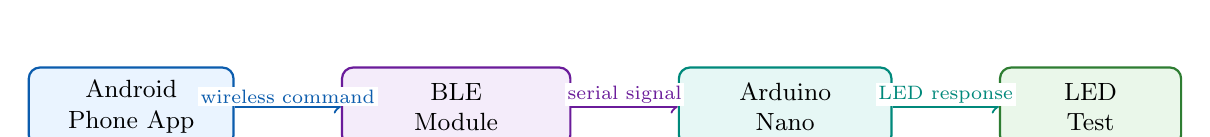
\begin{tikzpicture}[node distance=1.35cm, every node/.style={font=\small, align=center}]
  \node[draw=LabBlue, fill=LabLightBlue, rounded corners, thick, minimum width=2.6cm, minimum height=1.0cm] (phone) {Android\\Phone App};
  \node[draw=LabPurple, fill=LabLightPurple, rounded corners, thick, right=of phone, minimum width=2.9cm, minimum height=1.0cm] (ble) {BLE\\Module};
  \node[draw=LabTeal, fill=LabLightTeal, rounded corners, thick, right=of ble, minimum width=2.7cm, minimum height=1.0cm] (arduino) {Arduino\\Nano};
  \node[draw=LabGreen, fill=LabLightGreen, rounded corners, thick, right=of arduino, minimum width=2.3cm, minimum height=1.0cm] (led) {LED\\Test};
  \draw[->, thick, LabBlue] (phone) -- node[midway, above, fill=white, inner sep=1pt, font=\scriptsize]{wireless command} (ble);
  \draw[->, thick, LabPurple] (ble) -- node[midway, above, fill=white, inner sep=1pt, font=\scriptsize]{serial signal} (arduino);
  \draw[->, thick, LabTeal] (arduino) -- node[midway, above, fill=white, inner sep=1pt, font=\scriptsize]{LED response} (led);
\end{tikzpicture}
\end{center}

\section*{\textcolor{LabBlue}{3. Important Note About This Module}}

\colourbox{LabOrange}{LabLightOrange}{
  \textbf{\textcolor{LabOrange}{Special BLE Edition}}\\
  The module used in this lab looks like an HC-05 Bluetooth module, but it is a
  \textbf{special edition that works with BLE, not SPP}. SPP means Serial Port
  Profile, which is used by many classic Bluetooth HC-05 modules. This lab uses
  BLE, so students must use the provided Android app instead of a normal classic
  Bluetooth terminal app.
}

\begin{center}
  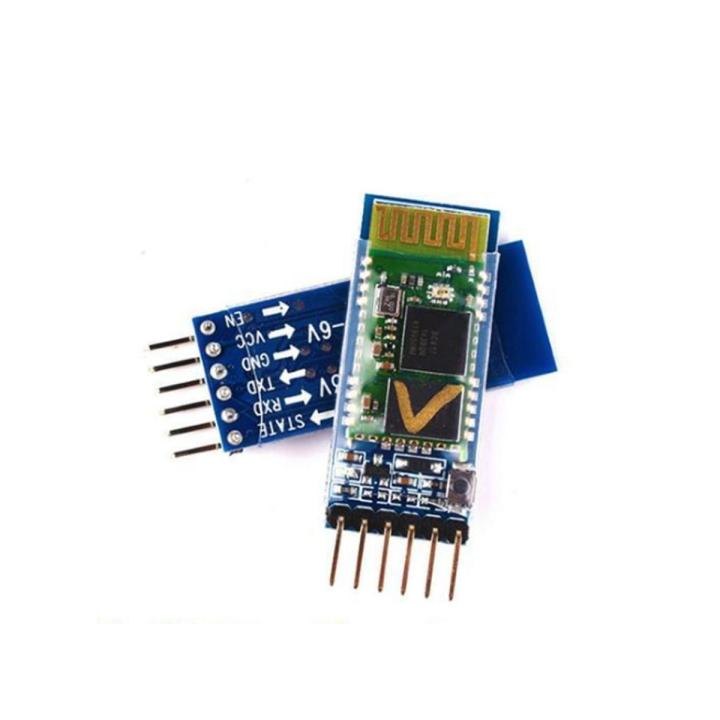
\includegraphics[width=0.36\linewidth]{assets/hc05_ble_module.jpg}\\[-0.2em]
  {\small \textbf{Bluetooth/BLE module used in this lab.} The pins are labelled
  EN, VCC, GND, TXD, RXD, and STATE.}
\end{center}

\section*{\textcolor{LabBlue}{4. Materials}}

\begin{tabularx}{\linewidth}{>{\bfseries}p{0.34\linewidth}X}
Arduino Nano ATmega168 & Receives wireless commands and runs the test code.\\
Special BLE HC-05-style module & Receives commands from the Android phone app.\\
Android phone & Runs the provided mobile app. iPhone is not supported in this lab.\\
USB cable & Uploads code and opens the Serial Monitor.\\
Jumper wires & Connect the module to the Arduino Nano.\\
Voltage divider resistors & Protect the module RXD pin from the Arduino's 5V TX signal.\\
\end{tabularx}

\section*{\textcolor{LabBlue}{5. Install the Android App}}

\colourbox{LabRed}{LabLightOrange}{
  \textbf{\textcolor{LabRed}{Android Only}}\\
  The mobile app for this lab works on \textbf{Android phones only}. It is not
  designed for iPhone.
}

\colourbox{LabPurple}{LabLightPurple}{
  \textbf{\textcolor{LabPurple}{Before Scanning for the Robot}}\\
  Make sure \textbf{Bluetooth} and \textbf{Location/GPS} are both turned on. The
  app must also have the required Android permissions for connectivity and
  location, such as Nearby Devices, Bluetooth, and Location permissions. Without
  these permissions, the app may not find the BLE module even if the wiring is
  correct.
}

Install the app from this link:

\begin{center}
\url{https://drive.google.com/file/d/10tnT_rNqe7tGeGTrUGqdO2R689uXVynw/view?usp=drive_link}
\end{center}

\begin{enumerate}
  \item Open the link on an Android phone.
  \item Download the app file.
  \item If Android asks for permission to install from this source, ask your instructor before continuing.
  \item Install the app.
  \item Open the app and keep it ready for the testing steps.
\end{enumerate}

\section*{\textcolor{LabBlue}{6. How the App Sends Commands}}

The app was created using MIT App Inventor. The app buttons send small command
values to the BLE module.

\begin{center}
  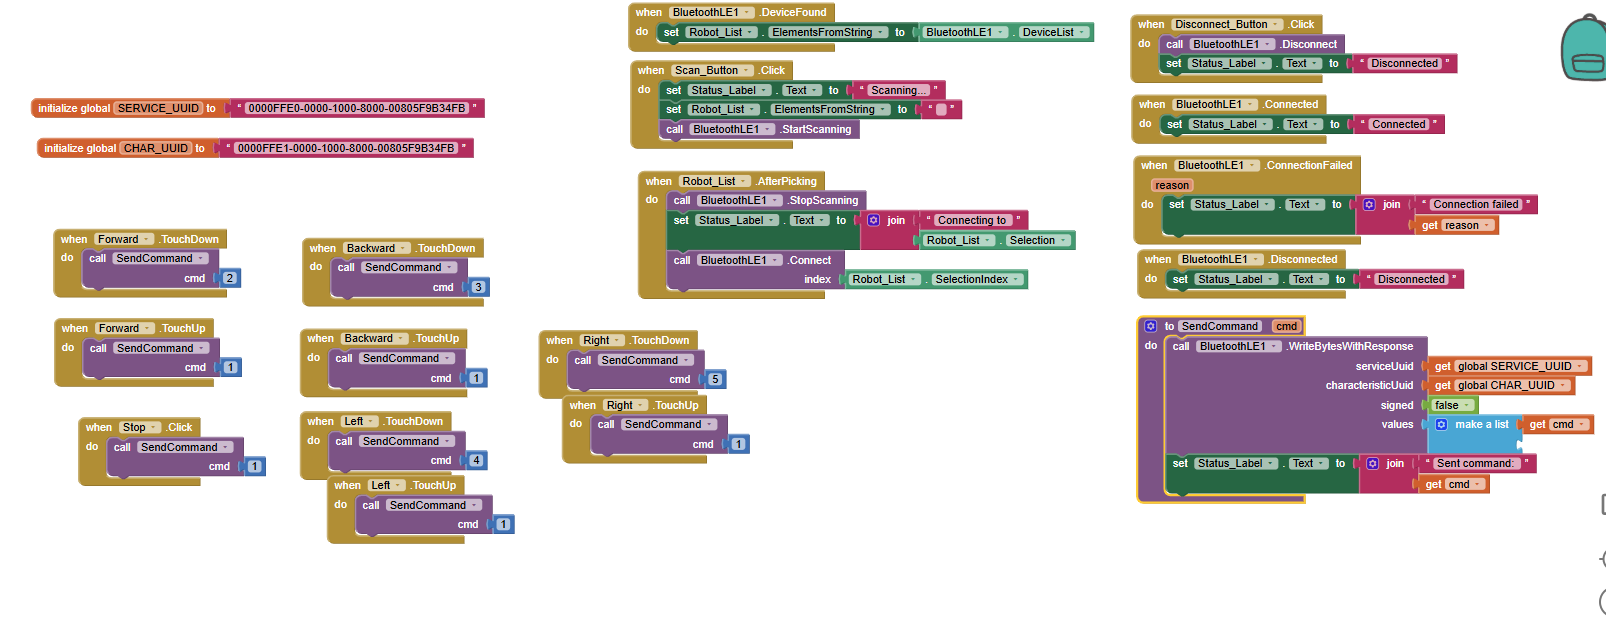
\includegraphics[width=\linewidth]{assets/app_blocks.png}\\[-0.2em]
  {\small \textbf{MIT App Inventor blocks.} The app scans for BLE devices,
  connects to the robot module, and sends command values when buttons are pressed.}
\end{center}

\begin{center}
\rowcolors{2}{LabLightTeal}{white}
\begin{tabular}{>{\centering\arraybackslash\bfseries}p{0.16\linewidth} p{0.46\linewidth} p{0.24\linewidth}}
\rowcolor{LabTeal}
\textcolor{white}{Command} & \textcolor{white}{Meaning} & \textcolor{white}{In This Test}\\
1 & Stop & LED OFF\\
2 & Forward & LED ON\\
3 & Backward & LED ON\\
4 & Left & LED ON\\
5 & Right & LED ON\\
\end{tabular}
\end{center}

\section*{\textcolor{LabBlue}{7. Wiring the BLE Module}}

\colourbox{LabRed}{LabLightOrange}{
  \textbf{\textcolor{LabRed}{Protect the RXD Pin}}\\
  The Arduino Nano sends 5V logic from D11. Many Bluetooth/BLE module RXD pins
  expect about 3.3V logic. Use a voltage divider between Arduino D11 and module
  RXD.
}

\begin{center}
\rowcolors{2}{LabLightBlue}{white}
\begin{tabular}{>{\bfseries}c c p{0.42\linewidth}}
\rowcolor{LabBlue}
\textcolor{white}{Module Pin} & \textcolor{white}{Arduino Nano Pin} & \textcolor{white}{Notes}\\
TXD & D10 & Module transmits to Arduino receive pin.\\
RXD & D11 & Use a voltage divider before RXD.\\
GND & GND & Must share ground with the Arduino.\\
VCC & 5V or 3.3V & Use the correct power for your module board.\\
EN & Not used & Leave unconnected for this lab.\\
STATE & Not used & Leave unconnected for this lab.\\
\end{tabular}
\end{center}

\begin{center}
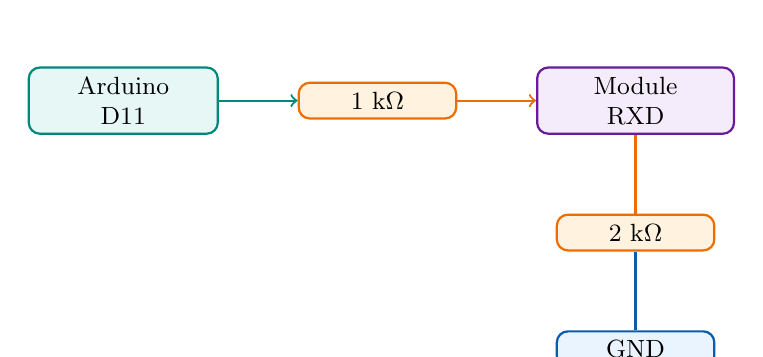
\begin{tikzpicture}[node distance=1cm, every node/.style={font=\small, align=center}]
  \node[draw=LabTeal, fill=LabLightTeal, rounded corners, thick, minimum width=2.4cm] (d11) {Arduino\\D11};
  \node[draw=LabOrange, fill=LabLightOrange, rounded corners, thick, right=of d11, minimum width=2.0cm] (r1) {1 k\(\Omega\)};
  \node[draw=LabPurple, fill=LabLightPurple, rounded corners, thick, right=of r1, minimum width=2.5cm] (rxd) {Module\\RXD};
  \node[draw=LabOrange, fill=LabLightOrange, rounded corners, thick, below=of rxd, minimum width=2.0cm] (r2) {2 k\(\Omega\)};
  \node[draw=LabBlue, fill=LabLightBlue, rounded corners, thick, below=of r2, minimum width=2.0cm] (gnd) {GND};
  \draw[->, thick, LabTeal] (d11) -- (r1);
  \draw[->, thick, LabOrange] (r1) -- (rxd);
  \draw[-, thick, LabOrange] (rxd) -- (r2);
  \draw[-, thick, LabBlue] (r2) -- (gnd);
\end{tikzpicture}\\[-0.2em]
{\small One simple voltage divider: Arduino D11 \(\rightarrow\) 1 k\(\Omega\)
\(\rightarrow\) module RXD, then module RXD \(\rightarrow\) 2 k\(\Omega\)
\(\rightarrow\) GND.}
\end{center}

\section*{\textcolor{LabBlue}{8. Arduino IDE Setup}}

\begin{enumerate}
  \item Open the Arduino IDE or PlatformIO project.
  \item Open the Lab 5 Part 1 code.
  \item Select \textbf{Tools \(\rightarrow\) Board \(\rightarrow\) Arduino AVR Boards \(\rightarrow\) Arduino Nano}.
  \item Select \textbf{Tools \(\rightarrow\) Processor \(\rightarrow\) ATmega168}.
  \item Select the correct \textbf{Tools \(\rightarrow\) Port}.
  \item Upload the code.
  \item Open \textbf{Tools \(\rightarrow\) Serial Monitor}.
  \item Set the baud rate to \textbf{9600}.
\end{enumerate}

\section*{\textcolor{LabBlue}{9. Experiment Procedure}}

\subsection*{\textcolor{LabTeal}{Part A: USB Test First}}

\begin{enumerate}
  \item Open the Serial Monitor at 9600 baud.
  \item Send \texttt{?}.
  \item Send \texttt{2}.
  \item Send \texttt{1}.
\end{enumerate}

\colourbox{LabGreen}{LabLightGreen}{
  \textbf{Observation:} What did the Serial Monitor print? What happened to the LED?\\[1.5em]
  \hrulefill
}

\subsection*{\textcolor{LabTeal}{Part B: Connect the Phone App}}

\begin{enumerate}
  \item Turn on Bluetooth and Location/GPS on the Android phone.
  \item Check that the app has Bluetooth/connectivity and Location permissions.
  \item Open the RoboLink app.
  \item Press the scan button in the app.
  \item Choose the BLE module from the list.
  \item Wait until the app says it is connected.
\end{enumerate}

\colourbox{LabPurple}{LabLightPurple}{
  \textbf{Connection observation:} What name appeared for your BLE module?\\[1.5em]
  \hrulefill
}

\subsection*{\textcolor{LabTeal}{Part C: Wireless Command Test}}

Press each app button and record what happens.

\begin{center}
\rowcolors{2}{LabLightBlue}{white}
\begin{tabularx}{\linewidth}{>{\bfseries}c X X}
\rowcolor{LabBlue}
\textcolor{white}{Command} & \textcolor{white}{Expected Result} & \textcolor{white}{What Actually Happened?}\\
1 / Stop & LED turns OFF & \\
2 / Forward & LED turns ON & \\
3 / Backward & LED turns ON & \\
4 / Left & LED turns ON & \\
5 / Right & LED turns ON & \\
\end{tabularx}
\end{center}

\section*{\textcolor{LabBlue}{10. What Is Happening in the Code?}}

\begin{tabularx}{\linewidth}{>{\bfseries}p{0.28\linewidth}X}
\texttt{SoftwareSerial} & Creates a second serial port on pins D10 and D11.\\
\texttt{bluetooth.begin(9600)} & Starts communication with the BLE module.\\
\texttt{bluetooth.available()} & Checks if the phone app sent a command.\\
\texttt{bluetooth.read()} & Reads one command from the BLE module.\\
\texttt{normalizeCommand()} & Makes raw byte commands, text digits, and lowercase letters easier to handle.\\
\texttt{handleCommand()} & Chooses what action to run for each command.\\
\texttt{digitalWrite(13, HIGH)} & Turns the built-in LED on.\\
\texttt{digitalWrite(13, LOW)} & Turns the built-in LED off.\\
\end{tabularx}

\section*{\textcolor{LabBlue}{11. Expected Problems and Fixes}}

\begin{center}
\rowcolors{2}{LabLightOrange}{white}
\begin{tabularx}{\linewidth}{>{\bfseries}p{0.25\linewidth}X X}
\rowcolor{LabOrange}
\textcolor{white}{Problem} & \textcolor{white}{Possible Cause} & \textcolor{white}{What To Try}\\
Phone cannot install app & Phone is not Android, or install permission is blocked & Use an Android phone and ask the instructor about install permission.\\
App cannot find module & BLE module is not powered, Bluetooth is off, Location/GPS is off, or app permissions are missing & Check VCC, GND, Bluetooth, Location/GPS, and app permissions.\\
App connects then fails & Wrong module type or weak power & Confirm this is the BLE special edition module and check power.\\
Serial Monitor shows nothing & Wrong baud rate or wrong port & Set Serial Monitor to 9600 and check Tools \(\rightarrow\) Port.\\
Upload fails & Wrong Nano processor setting & Select Tools \(\rightarrow\) Processor \(\rightarrow\) ATmega168.\\
Commands do nothing & TXD/RXD wiring is swapped or loose & Module TXD goes to D10. Arduino D11 goes to module RXD through voltage divider.\\
Module gets hot & Wiring or voltage is wrong & Disconnect power and ask the instructor to check the circuit.\\
\end{tabularx}
\end{center}

\section*{\textcolor{LabBlue}{12. Reflection Questions}}

Answer in full sentences.

\begin{enumerate}
  \item Why do we test wireless communication with the LED before connecting the motors?
  \vspace{2em}

  \item What is the difference between sending a command by USB Serial Monitor and sending it by BLE?
  \vspace{2em}

  \item Why does the Arduino D11 signal need a voltage divider before going to the module RXD pin?
  \vspace{2em}

  \item Why does this lab need the provided Android BLE app instead of a normal classic Bluetooth terminal app?
  \vspace{2em}

  \item If the app says it is connected but the Arduino receives nothing, what are two things you would check?
  \vspace{2em}
\end{enumerate}

\section*{\textcolor{LabBlue}{13. Exit Ticket}}

\colourbox{LabBlue}{LabLightBlue}{
  \textbf{In one or two sentences:} What did you learn about how a phone can send commands to a robot?\\[3em]
  \hrulefill\\[1.5em]
  \hrulefill
}

\section*{\textcolor{LabBlue}{14. Teacher Check}}

\colourbox{LabTeal}{LabLightTeal}{
  \textbf{\textcolor{LabTeal}{Teacher Checklist}}\\[0.4em]
  \begin{tabularx}{\linewidth}{>{\bfseries}p{0.58\linewidth}X}
    \checkboxitem{Wiring checked} & Notes: \hrulefill\\[1.0em]
    \checkboxitem{Code uploaded} & Notes: \hrulefill\\[1.0em]
    \checkboxitem{Android app installed} & Notes: \hrulefill\\[1.0em]
    \checkboxitem{BLE module connected in app} & Notes: \hrulefill\\[1.0em]
    \checkboxitem{Arduino receives wireless commands} & Notes: \hrulefill\\[1.0em]
    \checkboxitem{Students completed reflection questions} & Notes: \hrulefill\\
  \end{tabularx}
}

\end{document}
